\documentclass[../main.tex]{subfiles}

\begin{document}

\section{Neutrinos}%
\label{sec:neutrinos}

Als bijnaam hebben de neutrinos de naam ``ghost'' particles. De reden hiervoor is dat ze alleen zwak interageren wat hen een kleine werkzame doorsnede geeft en dus moeilijk te detecteren zijn. Bij deze deeltjes hebben we een hoop vragen die nog niet opgelost zijn.
\begin{itemize}
    \item Zijn dit Dirac of Majorana fermionen?
    \item Wat is hun massa?
    \item Wat zijn hun oscillatie eigenschappen?
    \item Is er $CP$ schending in de lepton sector?
    \item Zijn er rechts handige neutrinos?
    \item Zijn er meer dan 3 types neutrinos?
\end{itemize}
Vandaag de dag hebben we enkel een antwoord op de vraag wat hun oscillatie eigenschappen zijn. Dit alles zullen we bespreken in dit hoofdstuk.

\subsection{Neutrino bronnen}%
\label{sub:neutrino_bronnen}

Door het moeilijk te detecteren zijn is het belangrijk dat we er veel aanmaken. De belangrijkste bronnen zijn:
\begin{itemize}
    \item Zonne neutrinos: Ontstaan uit nucleaire reacties in de zon en dus met een energie in de MeV's. Om te zien hoe de zon neutrinos maakt moeten we kijken naar hoe deze brandt. De zon zal protonen fuseren tot $^4He$ kernen ($pp$-cyclus).
        \begin{equation}
            \begin{aligned}
                \label{eq:zon_fusie}
                p+p & \rightarrow D+e^{+}+\nu_{e} \\
                D+p & \rightarrow{ }^{3} \mathrm{He}+\gamma \\
                { }^{3} \mathrm{He}+{ }^{3} \mathrm{He} & \rightarrow{ }^{4} \mathrm{H}{ }^{2}+p+p
            \end{aligned}
        \end{equation}
        We moeten hier uiteindelijk 4 protonen omzetten in 2 protonen en 2 neutronen. Dit omzetten kan enkel gebeuren via de zwakke wisselwerking. We mogen blij zijn dat de zon zal branden aan de hand van de zwakke wisselwerking omdat deze anders heel snel opgebrand zou zijn. Naast deze $pp$-cyclus hebben we ook nog de Boron-cycle
        \begin{equation}
            \begin{aligned}
                \label{eq:boron_cyclus}
                { }^{4} \mathrm{He}+{ }^{3} \mathrm{He} & \rightarrow{ }^{7} \mathrm{Be}+\gamma \\
                { }^{7} \mathrm{Be}+p & \rightarrow{ }^{8} \mathrm{~B}+\gamma \\
                { }^{8} \mathrm{~B} & \rightarrow{ }^{8} \mathrm{Be}^{*}+e^{+}+\nu_{e} \\
                { }^{8} \mathrm{Be}^{*} & \rightarrow{ }^{4} \mathrm{He}+{ }^{4} \mathrm{He}
            \end{aligned}
        \end{equation}
        waar terug een zwakke wisselwerking component zit, de Be-capture
        \begin{equation}
            \begin{aligned}
                \label{eq:be_capture}
                { }^{7} \mathrm{Be}+e^{-} \rightarrow^{7} \mathrm{Li}+\nu_{e}
            \end{aligned}
        \end{equation}
        wat een zwakke wisselwerking is en de $pep$ reactie
        \begin{equation}
            \begin{aligned}
                \label{eq:pep}
                p+e^{-}+p \rightarrow D+\nu_{e}
            \end{aligned}
        \end{equation}
        De 2 laatste processen zullen een non energetisch neutrino aanmaken. Zo ziet het neutrino spectrum er als volgt uit.

        \begin{figure}[h]
            \centering
            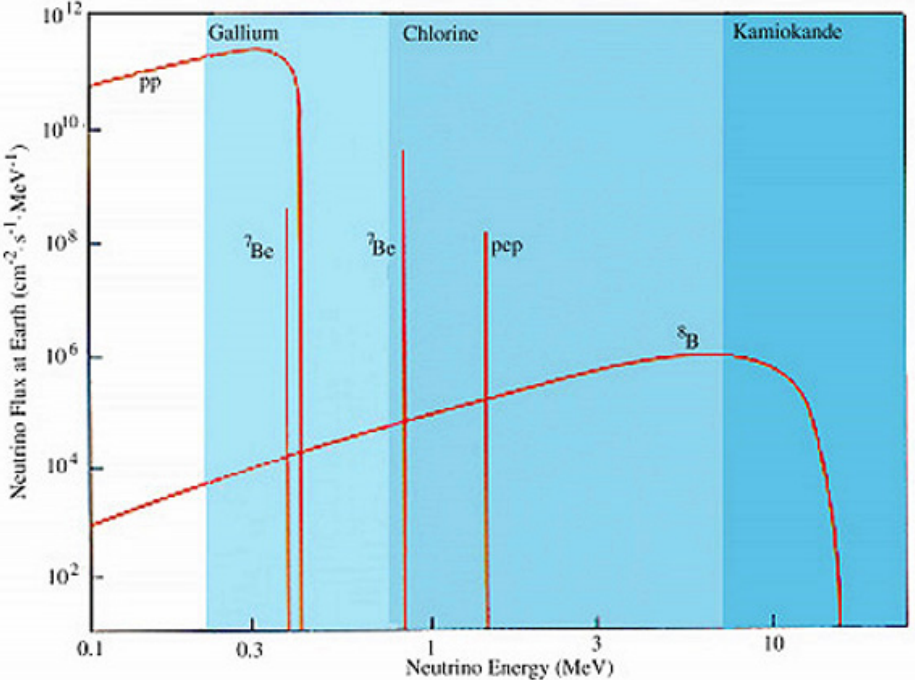
\includegraphics[width=0.5\linewidth]{neutrinos/zon_neutrino_spectrum.png}
            \caption{Spectrum van de zon neutrinos}%
            \label{fig:neutrinos/zon_neutrino_spectrum}
        \end{figure}

    \item Atmosferische neutrinos: Ontstaan uit hoog energetische reacties van kosmische straling die botst op de atmosfeer. De orde van de energie van deze neutrinos is in de GeV-PeV. De invallende protonen van kosmische straling hebben zo een hoge energie ($10^{21}$eV=$1$ZeV) dat we dit het ``Oh My God particle''. Deze bostsen op de atmosfeer die van alle soorten deeltjes geven die kunnen vervallen naar hoog energetische neutrinos. Dit gebeurt typisch op 15 kilimeter hoog.

        \begin{figure}[h]
            \centering
            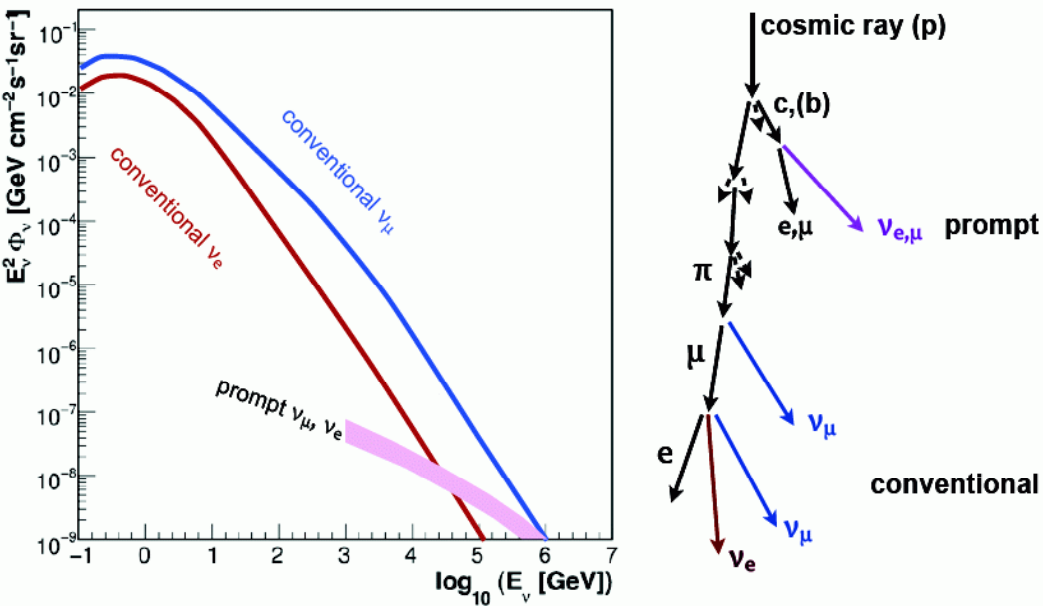
\includegraphics[width=0.5\linewidth]{neutrinos/kosmisch verval.png}
            \caption{Verval van kosmische straling in de atmosfeer}%
            \label{fig:neutrinos/kosmisch verval}
        \end{figure}

    \item Kern reactoren: Deze hebben energie in de orde van MeV's. In de nucleaire reactoren zijn er een hoop kernen aanwezig met een overmaat aan neutronen. Deze zetten een kettingreactie in gang waar de ene na de andere neutron rijke kern aan fissie productie doet. Dit is een $\beta^-$ verval $n \rightarrow p+e^{-}+\bar{\nu}_{e}$.
    \item Neutrino bundels: Deze worden gemaakt uit het verval van pion bundels $\pi \rightarrow \mu+\nu_{\mu} \rightarrow e+2 \nu_{\mu}+\nu_{e}$. De orde van de energie is in de GeV's.
\end{itemize}

\subsection{Zonne neutrino detectoren}%
\label{sub:zonne_neutrino_detectoren}

De allereerste detector om neutrinos te detecteren maakt gebruik van de het invers $\beta^-$ verval ($\bar{v}_{e}+p\rightarrow e^{+}+n$). In 1964 wordt dit geimplementeerd in het Homestake mine experiment. John Bacall is een theoretische astrofysicus die in detail uitrekende hoeveel neutrinos er uit de zon zouden moeten komen. Hij schat dat er enkele duizenden tot tienduizenden neutrinos per cm$^2$/s zouden moeten vrijkomen. Samen met Davis proberen ze dit nu te berekenen. Zoals gewoonlijk wordt dit voorstel afgewezen omdat het niet meetbaar zou zijn. Na bewijs dat het weldegelijk meetbaar is wordt het een 2de keer afgewezen omdat ze zeggen dat we toch weten uit berekeningen hoeveel neutrinos er uit de zon komen. Ze zijn hier toch mee verder gegaan met een groot vat aan droogkuisproduct. Hier zit chloor in dat de neutrinos kan opvangen.
\begin{equation}
    \begin{aligned}
        \label{eq:cl_neutrino_capture}
        \nu_{e}+^{37} \mathrm{Cl} \rightarrow^{37} \mathrm{Ar}+e^{-}
    \end{aligned}
\end{equation}
De threshold voor deze reactie is $E_\nu > 0.814$MeV. Het zou makkelijker zijn om het elektron van deze reactie te meten in plaats van het bubbeltje aan argon gas maar er zijn zo weinig evenementen dat het zo goed als onmogelijk is om deze waar te nemen.
\begin{equation}
    \begin{aligned}
        \label{eq:homestake_mine_exp}
        R(\mathrm{Cl}, S S M) &=8.1 \pm 1.3 S N U \\
        R(\mathrm{Cl}, \text { exp. }) &=2.56 \pm 0.16 \pm 0.16 S N U
    \end{aligned}
\end{equation}
$SNU$ is hier de solar neutrino unit. De foutenvlag van het standaard zonne model komt van de onzekerheden van de astrofysische modelen die we hebben van de zon. In het experiment zien we maar $30\%$ van de voorspelde neutrino flux.\\
De reacties hierop zijn voorspelbaar. Langs de ene kant wordt door theoretischi gezegd dat ze niet kunnen meten en de experimenticussen zeggen dat een slechte voorspelling is gemaakt. Als je zo een verschil ziet, probeer je het experiment opnieuw maar beter uit te voeren om zeker te zijn wat we hebben waargenomen.\\
Het is beter om dit experiment met gallium capture van neutrinos uit te voeren.
\begin{equation}
    \begin{aligned}
        \label{eq:ga_neutrino_capture}
        \nu_{e}+{ }^{71} \mathrm{Ga} \rightarrow{ }^{71} \mathrm{Ge}+e^{-}
    \end{aligned}
\end{equation}
Het voordeel bij deze reactie is dat de energie threshold kleiner is, $E_\nu = 0.233$MeV. Met deze threshold is het mogelijk om neutrinos uit de $pp$-cyclus waar te nemen. Het probleem bij dit experiment is dat gallium niet makkelijk te verkrijgen is en dus duur is. Dit onderzoek is gedaan in het GALLEX en SAGE experiment. SAGE staat voor soviet american gallium experiment. In 1992 is de Soviet unie gevallen en was het te gevaarlijk geworden om het SAGE experiment verder te zetten in het Caucasus gebergte. Het heeft geduurd tot eind  de jaren 90 om de zaken terug onder controle te krijgen. Hieruit kregen we terug dat er te weinig neutrinos werden waargenomen.\\
Het probleem bij dit soort experimenten was dat enkel het aantal waargenomen neutrinos werd geteld, niet hun richting. We waren dus niet zeker dat deze neutrinos van de zon kwamen. Het is dus nodig een experiment te ontwerpen die dit wel kan. Het Kamiokande experiment probeert de neutrinos waar te nemen aan de hand van elastische botsingen, $\nu_{x}+e^{-} \rightarrow \nu_{x}+e^{-}$. Hier is een gigantische hoeveelheid ultra zuiver water waar een elektron kan versneld worden aan de hand van de elastische botsing. Dit elektron zal in het water sneller dan het licht gaan en doet aan Cerenkov straling. Projecteer je deze straling op een detector dan krijg je Cerenkov ringen. Aan de hand van de grote van de ring kan een idee gekregen worden over de snelheid van het elektron. Belangrijker kan aan de hand van de oriëntatie van deze ring de richting van het elektron bepaald worden. Het nadeel hierbij is dat er hoge threshold energie nodig is. Zetten we het aantal evenementen nu uit in functie van de hoek naar de zon (figuur \ref{fig:neutrinos/kamiokande_results}) zien we duidelijk dat er een overschot is aan neutrinos die komen van de zon.

\begin{figure}[h]
    \centering
    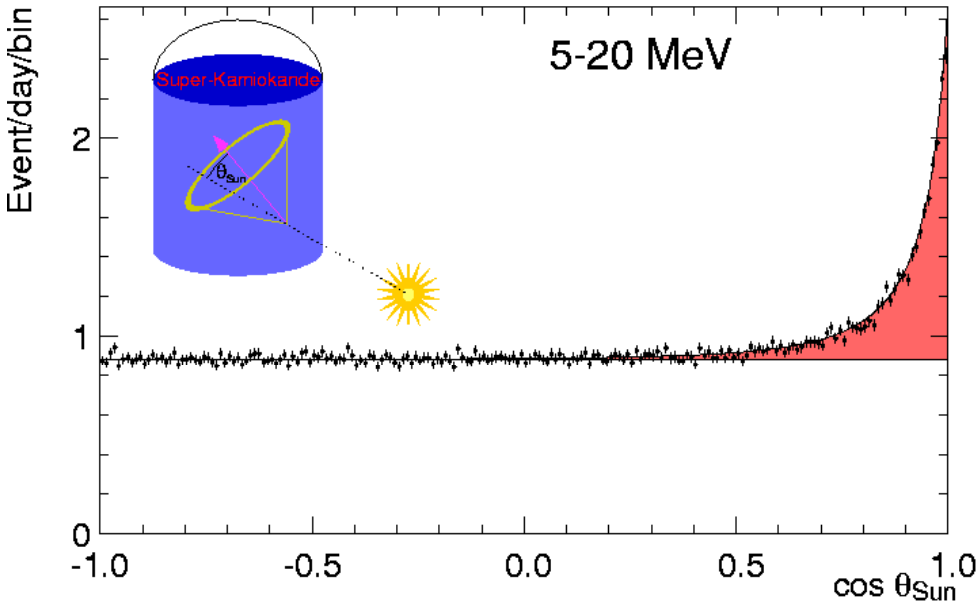
\includegraphics[width=0.5\linewidth]{neutrinos/kamiokande_results.png}
    \caption{Resultaten van het Kamiokande experiment}%
    \label{fig:neutrinos/kamiokande_results}
\end{figure}

Bekijken we nu alle resultaten van deze experimenten samen:
\begin{equation}
    \begin{aligned}
        \label{eq:zonne_neutrino_resultaten}
        R(\mathrm{Cl}, S S M) &=8.1 \pm 1.3 S N U \\
        R(\mathrm{Cl}, \text { exp. }) &=2.56 \pm 0.16 \pm 0.16 S N U \\
        R(\mathrm{Ga}, S S M) &=126 \pm 10 S N U \\
        R(\mathrm{Ga}, G A L L E X) &=69.3 \pm 4.1 \pm 3.6 S N U \\
        R(\mathrm{Ga}, S A G E) &=70.8_{-5.2-3.2}^{+5.3+3.7} S N U \\
        \Phi_{S S M} &=(5.69 \pm 0.91) \times 10^{10} \text{m}^{-2} \text{s}^{-1} \\
        \Phi_{S K} &=(2.35 \pm 0.02 \pm 0.08) \times 10^{10} \text{m}^{-2} \text{s}^{-1}
    \end{aligned}
\end{equation}
Zoals bij het initiële zonne neutrino experiment is er in GALLEX en SAGE experiment ook een tekort gevonden met maar $70\%$ van de hoeveelheid voorspelde neutrinos waargenomen. Hetzelfde voor Kamiokande vinden we maar $1/2$ van de voorspelde neutrinos. Uit deze resultaten concluderen we dat een deel van de neutrinos verdwijnen onderweg van het centrum van de zon tot ons.\\
Een mogelijkheid zou zijn dat de zon is gestopt met branden. De reden waarom dat mogelijk is, is omdat het 10000 jaar zou duren voor de energie, protonen, elektronen... om van het centrum van de zon naar de rand te geraken. Daarentegen zullen de centrale neutrinos hier zijn in 8 minuten. Zo is het mogelijk dat we het stoppen van het branden van het centrum van de zon wel al kunnen zien in de neutrinos maar niet aan de zon zelf. Dit is een absurde stelling die we niet echt in acht moeten nemen.

\subsection{SNO (=Sudbury Neutrino Observatory)}%
\label{sub:sno}

Waar de neutrinos naartoe gaan, wordt aangetoond in 2002 in het SNO experiment.

\begin{figure}[h]
    \centering
    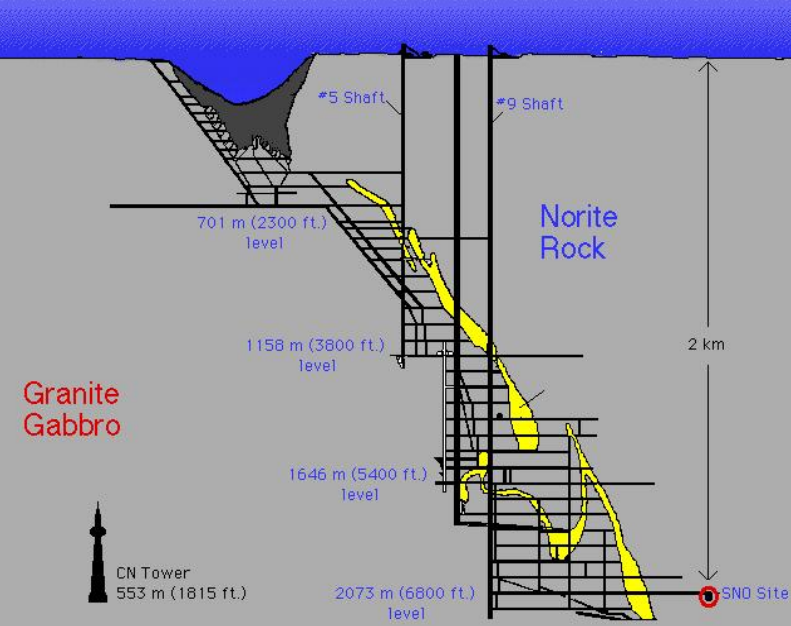
\includegraphics[width=0.5\linewidth]{neutrinos/sno_schematisch.png}
    \caption{Schematische voorstelling van het SNO experiment}%
    \label{fig:neutrinos/sno_schematisch}
\end{figure}

\begin{figure}[h]
    \centering
    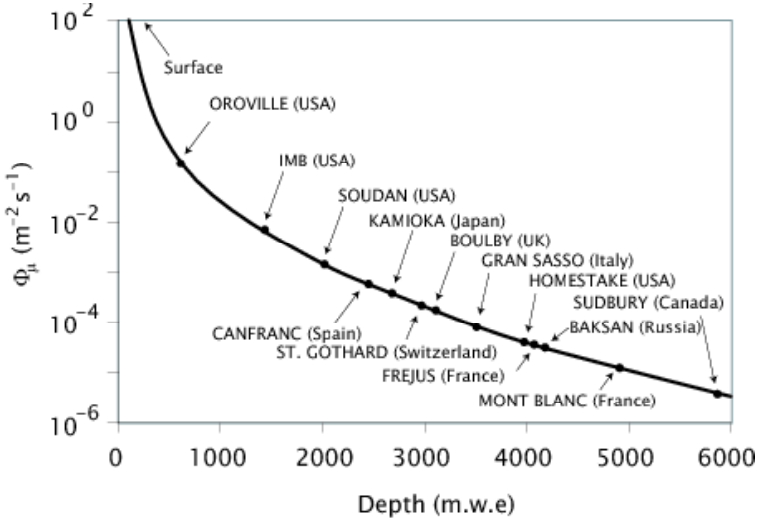
\includegraphics[width=0.5\linewidth]{neutrinos/muon_achtergrond_verval.png}
    \caption{Muon achtergrond in functie van de diepte}%
    \label{fig:neutrinos/muon_achtergrond_verval}
\end{figure}

Het SNO laboratorium is een clean room 2 kilometer onder de grond in een mijn. De reden waarom we zo diep onder de grond gaan is om de muon achtergrond van kosmische straling, waar deze detectoren heel gevoelig voor zijn, te minimaliseren. Het speciale aan deze detector was het gebruik van zwaar water in de Cerenkov detector. Wat zijn nu de mogelijke interacties die kunnen plaats vinden in deze detector.
\begin{itemize}
    \item elastische botsingen: $\nu_{x}+e^{-} \rightarrow \nu_{x}+e$
    \item charged current reactie: $\nu_{e}+D \rightarrow p+p+e^{-}$
    \item neutral curent reactie: $\nu_{x}+D \rightarrow p+n+\nu_{x}$
\end{itemize}
De geladen reactie zal niet genoeg energie hebben om een muon aan te maken, de andere reacties zijn wel gevoelig aan alle flavours met de elastische botsing gevoeliger voor elektronen omdat deze meer feynman diagrammen hebben.
\begin{equation}
    \begin{aligned}
        \label{eq:sno_flavour_gevoeligheid}
        \mathrm{CC} &\propto \phi\left(\nu_{e}\right) \\
        \mathrm{NC} &\propto \phi\left(\nu_{e}\right)+\phi\left(\nu_{\mu}\right)+\phi\left(\nu_{\tau}\right) \\
        \mathrm{ES} &\propto \phi\left(\nu_{e}\right)+0.154\left[\phi\left(\nu_{\mu}\right)+\phi\left(\nu_{\tau}\right)\right]
    \end{aligned}
\end{equation}
Nu we weten wat er hier gebeurt, kunnen we de resultaten van dit experiment bekijken.

\begin{figure}[h]
    \centering
    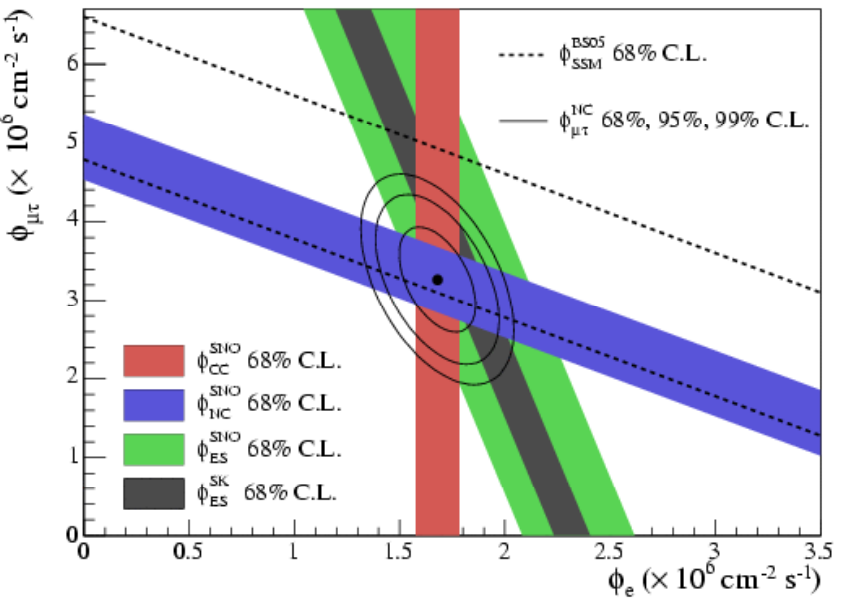
\includegraphics[width=0.5\linewidth]{neutrinos/sno_resultaten.png}
    \caption{Resultaten van SNO experiment}%
    \label{fig:neutrinos/sno_resultaten}
\end{figure}

In deze resultaten hebben we horizontaal de flux aan elektro neutrinos en verticaal de flux aan muon en tau neutrinos. In het rood zien we wat de charge current reactie geeft, die natuurlijk enkel flux voor elektronen geeft. Deze flux is veel lager dan wat we verwachten in het Standaard Model. Deze zouden voor het Standaard model buiten de figuur liggen. In het blauw zien we de resultaten van de neutral current reacties wat de sommatie is van de verschillende neutrinos samen is. Wat mooi is dat deze neutrinos samen wel het standaard model (stippellijnen in grafiek) volgen. Al de metingen die gedaan zijn komen samen tot 1 punt waar we zien dat maar $1/3$ van de neutrinos van de zon bestaan uit $\nu_e$.\\
Hiermee hebben we ten eerste bewezen dat we begrijpen hoe dat de zon werkt op enkele procenten na, ten tweede dat de neutrinos er wel degelijk uitkomen en dat we ze kunnen detecteren en ten derde dat de neutrinos aangemaakt worden als $\mu_e$ maar onderweg opmengen met de andere flavours, ze zijn er in geoscilleerd.

\subsection{KamLAND}%
\label{sub:kamland}

Verder bewijs van deze oscillaties komt in 2002 in het KamLAND experiment (Kamioka Liquid Scintillator Anti-Neutrino
Detector). Hier wordt er gekeken naar $\bar{\nu}_e$ antineutrinos afkomstig van een Japanse en Zuid-Koreaanse kern centrales met een gemiddelde afstand van $L\approx180$km. Van al de reactoren die ze gebruiken kunnen ze aan de hand van hun vermogen bepalen hoeveel antineutrinos moeten vrij komen. De detector maakt gebruik van een vloeibare scintillator waar aan elastische verstrooiing kan gedaan worden $\bar{\nu}_{e}+e^{-} \rightarrow \bar{\nu}_{e}+e^{-}$. De bewegende elektronen zullen kunnen getracked worden in de scintillator. Omdat we de energie van de elektronen te kunnen bepalen is het mogelijk om het spectrum van neutrinos te bepalen.

\begin{figure}[h]
    \centering
    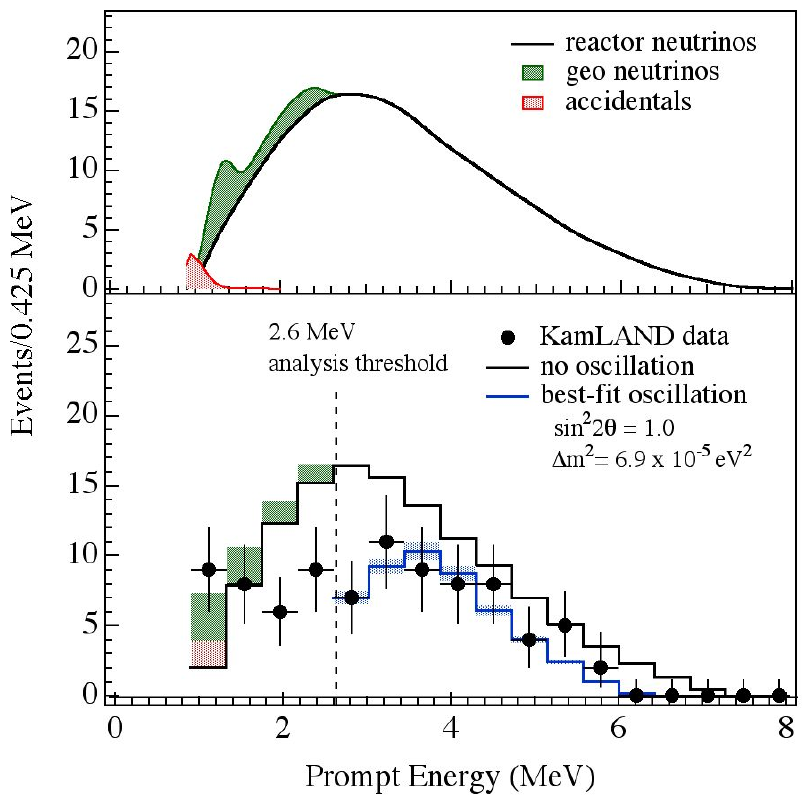
\includegraphics[width=0.5\linewidth]{neutrinos/kamland_results.png}
    \caption{Energie spectrum van neutrinos in KamLAND}%
    \label{fig:neutrinos/kamland_results}
\end{figure}

De Bovenste grafiek toont het spectrum dat we verwachten uit de theorie. Naast in het zwart de neutrinos van de reactoren in het zwart en de achtergrond in het rood verwachten we nog een interessant soort neutrinos te vinden, de geo neutrinos. Dit zijn neutrinos die ontstaan in de aarde van radioactieve kernen aanwezig in de aarde. De extra hoeveelheid warmte dat de aarde uitstraalt dat niet van de zon komt moet komen van dit radioactief verval binnenin de aarde. In de onderste grafiek kunnen we de theorie omgevormd tot het zwarte diagram. Wat we waarnemen zijn de zwart stippen wat helemaal anders is. Zetten we de overleving probabiliteit van de neutrinos nu uit in functie van de ratio van de afgelegde afstand op zijn energie dan krijg je figuur \ref{fig:neutrinos/kamland_osc}.

\begin{figure}[h]
    \centering
    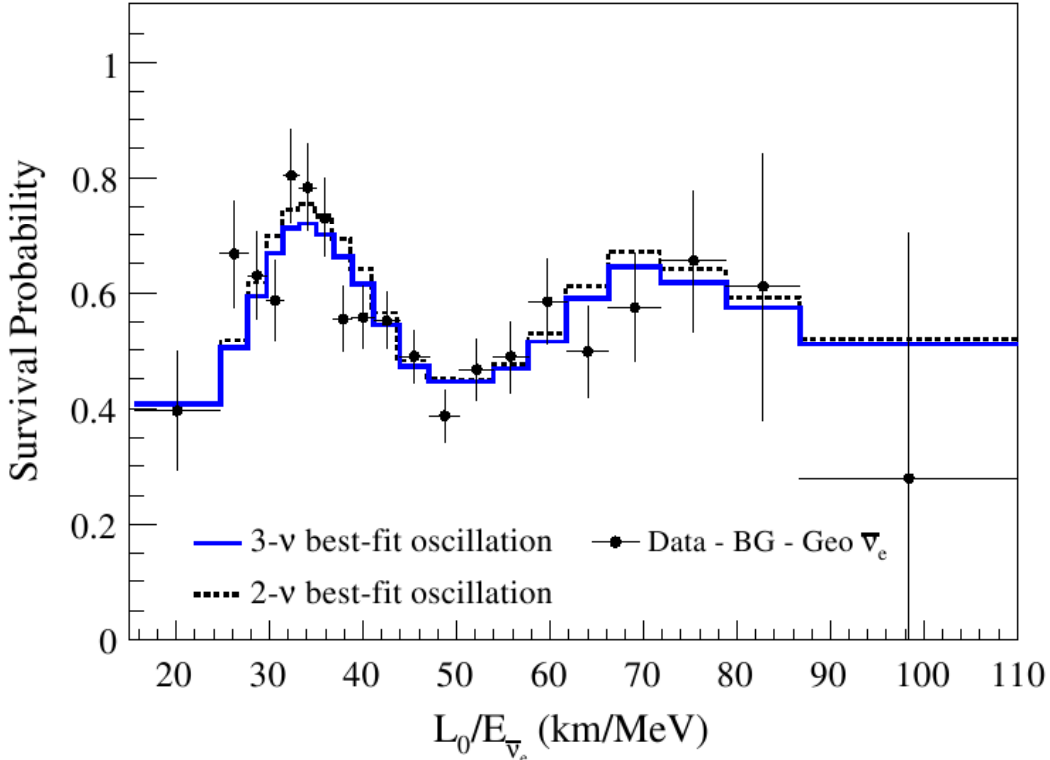
\includegraphics[width=0.6\linewidth]{neutrinos/kamland_osc.png}
    \caption{Overleving probabiliteit in functie van de afstand en energie}%
    \label{fig:neutrinos/kamland_osc}
\end{figure}

In deze uitzetting kan je mooi zien dat de antineutrinos oscilleren.

\subsection{Oscillaties: 2 generaties}%
\label{sub:oscillaties_2_generaties}

Om het onszelf makkelijk te houden op dit moment, kijken we alleen naar oscillaties tussen 2 generaties, $\nu_e$ en $\nu_\mu$. De massaeigentoestanden kennen we uit de Schrödinger vergelijking. Deze gedragen zich als een vlakke golf.
\begin{equation}
    \begin{aligned}
        \label{eq:massa_eigentoestanden_neutrinos}
        \left|\nu_{i}(t)\right>=\left| \nu_{i}\right>e^{i\left(\vec{p}_{i} \cdot \vec{x}-E_{i} t\right)}=\left| \nu_{i}\right>e^{-i \phi_{i}}
    \end{aligned}
\end{equation}
Omdat $\vec{p}_{i} \cdot \vec{x}-E_{i} t$ vrij lang is om op te schrijven hebben we dit samengevoegd in een fase $\phi_i$. De relatie tussen de massa eigentoestanden en flavour eigentoestanden is weer niets anders dan een rotatie over de hoek $\theta$. Wat gebeurt er hier nu? We creëren in reacties flavour eigentoestanden. Omdat deze neutrinos geen lading hebben zullen deze opmengen met elkaar.
\begin{equation}
    \begin{aligned}
        \label{eq:neutrino_2_gen_opmenging}
        \left(\begin{array}{c}
                \nu_{e} \\
                \nu_{\mu}
                \end{array}\right)=\left(\begin{array}{cc}
                \cos \theta & \sin \theta \\
                -\sin \theta & \cos \theta
                \end{array}\right)\left(\begin{array}{l}
                \nu_{1} \\
                \nu_{2}
        \end{array}\right)
    \end{aligned}
\end{equation}
Indien dat de fases van de verschillende massa eigentoestanden gelijk zijn, zijn er geen oscillaties. Dit is het geval in het Standaard Model omdat neutrinos daar geen massa hebben. In tegenstrijd met het Standaard Model hebben we waargenomen dat neutrinos wel massa hebben en dus zullen oscilleren. Gaan we ervan uit dat we ons op $t=0$ in een pure neurtrino $\nu_e$ toestand bevinden.
\begin{equation}
    \begin{aligned}
        \label{eq:neutrino_2_oscilaties_1}
        \left|\psi(0)\right>=\cos \theta\left| \nu_{1}\right>+\sin \theta \left| \nu_{2}\right>
    \end{aligned}
\end{equation}
Na tijd $T$ op afstand $L$ hebben we:
\begin{equation}
    \begin{aligned}
        \label{eq:neutrino_2_oscilaties_2}
        \left|\psi(L, T)\right>=\cos \theta\left| \nu_{1}\right>e^{-i \phi_{1}}+\sin \theta \left| \nu_{2}\right>e^{-i \phi_{2}}
    \end{aligned}
\end{equation}
Hierbij hebben we voor elke massa eigentoestand een verschillende fase. Schrijven we dit nu uit in functie van de flavour eigentoestanden aan de hand van vergelijking (\ref{eq:neutrino_2_gen_opmenging}):
\begin{equation}
    \begin{aligned}
        \label{eq:neutrino_2_oscilaties_3}
        \left|\psi(L, T)\right>=\left(e^{-i \phi_{1}} \cos ^{2} \theta+e^{-i \phi_{2}} \sin ^{2} \theta\right)\left| \nu_{e}\right>\\
        -\left(e^{-i \phi_{1}}-e^{-i \phi_{2}}\right) \cos \theta \sin \theta \left| \nu_{\mu}\right>
    \end{aligned}
\end{equation}
We hebben nu aangetoond dat we na zekere tijd een opmenging krijgen met $\nu_\mu$ met als voorwaarde dat $\theta\neq 0$ en de fases niet gelijk zijn. Dit verschil in fase is enkel mogelijk als er een verschil in massa is. Rekenen we dit verder uit dan krijgen we:
\begin{equation}
    \begin{aligned}
        \label{eq:neutrino_2_oscilaties_4}
        \left|\psi(L, T)\right>=& e^{-i \phi_{1}}\left[\left(\cos ^{2} \theta+e^{i \Delta \phi_{12}} \sin ^{2} \theta\right)\left|\nu_{e}\right>\right.\\
                                &\left.-\left(1-e^{i \Delta \phi_{12}}\right) \cos \theta \sin \theta\left|\nu_{\mu}\right>\right] \\
        =& c_{e}\left|\nu_{e}\right>+c_{\mu}\left| \nu_{\mu}\right>
    \end{aligned}
\end{equation}
We verkrijgen dus een zekere waarschijnlijkheid $c_e^2$ om $\nu_e$ te krijgen en om $\nu_\mu$ te krijgen $c_\mu^2$. De waarschijnlijkheid om $\nu_e$ om te zetten in een $\nu_\mu$ is gegeven door:
\begin{equation}
    \begin{aligned}
        \label{eq:neutrino_2_oscilaties_5}
        P\left(\nu_{e} \rightarrow \nu_{\mu}\right) &=c_{\mu} c_{\mu}^{*}=\left(1-e^{i \Delta \phi_{12}}\right)\left(1-e^{-i \Delta \phi_{12}}\right) \cos ^{2} \theta \sin ^{2} \theta \\
                                                    &=\sin ^{2}(2 \theta) \sin ^{2}\left(\frac{\Delta \phi_{12}}{2}\right)\\
        \Delta \phi_{12}&=\left(E_{1}-E_{2}\right) T-\left(p_{1}-p_{2}\right) L
    \end{aligned}
\end{equation}
Het is terug duidelijk dat $\theta\neq 0$ en dat er een faseverschil moet zijn om opmenging te kunnen krijgen. Het verder uitwerken van de dit faseverschil moet normaal gedaan worden aan de hand van golf pakket propagatie. Wat er uiteindelijk gebeurt, is de generatie van een golfpacket bij $t=0$ dat je identificeert als een elektron neutrino. Dat golfpacket propageert zich in de tijd op een niet triviale manier beschreven door de Schrödinger vergelijking. Deze golfvergelijking zal op een bepaalt moment interageren met de golffunctie van de kern om het golfpakket te detecteren. Dit zou allemaal op een heel propere manier moeten uitgewerkt worden. Dit alles kan benadert worden met als voorwaarde dat de productie en detectie op groot genoege afstand van elkaar gebeuren zodat het golfpakket als een vlakke golf kan benadert worden. Indien we dit doen en we stellen $p_{1}=p_{2}=p$ of $E_{1}=E_{2}=E$ of $\beta_{1}=\beta_{2}=\beta$ gelijk aan elkaar, dan leiden ze allemaal tot dezelfde faseverschil:
\begin{equation}
    \begin{aligned}
        \label{eq:neutrino_2_oscilaties_6}
        \Delta \phi_{12}=\left(E_{1}-E_{2}\right) T &=\left[p\left(1+\frac{m_{1}^{2}}{p^{2}}\right)^{\frac{1}{2}}-p\left(1+\frac{m_{2}^{2}}{p^{2}}\right)^{\frac{1}{2}}\right] T \\
                                                    & \approx \frac{m_{1}^{2}-m_{2}^{2}}{2 p} L
    \end{aligned}
\end{equation}
Dit resultaat zal ook bekomen worden voor de mooie uitwerking met golf pakket propagatie. Nu we dit hebben kunnen we de waarschijnlijkheden van de opmengingen verder uitwerken:
\begin{equation}
    \begin{aligned}
        \label{eq:neutrino_2_oscilaties_7}
        P\left(\nu_{e} \rightarrow \nu_{\mu}\right) &=\sin ^{2}(2 \theta) \sin ^{2}\left(\frac{\left(m_{1}^{2}-m_{2}^{2}\right) L}{4 E_{\nu}}\right) \\
                                                    &=\sin ^{2}(2 \theta) \sin ^{2}\left(1.267 \frac{\Delta m^{2}\left[\mathrm{eV}^{2}\right] L[\mathrm{~km}]}{E_{\nu}[\mathrm{GeV}]}\right) \\
        P\left(\nu_{e} \rightarrow \nu_{e}\right) &=1-\sin ^{2}(2 \theta) \sin ^{2}\left(\frac{\left(m_{1}^{2}-m_{2}^{2}\right)^{2} L}{4 E_{\nu}}\right)
    \end{aligned}
\end{equation}
De factor $1.267$ komt van het omzetten in de verschillende eenheden. Zoals bij de meson oscillaties zien we nu terug een afhankelijkheid van de oscillaties aan het massaverschil van de neutrinos maar deze is niet helemaal hetzelfde. Bij de mesonen hebben we een factor $\Delta m\cdot t$, hier hebben wen $\Delta m^2$ zonder een tijd afhankelijkheid. Van waar komt dit verschil? We hebben dezelfde berekeningen uitgevoerd. Het verschil zit hem in de initiële fase $\vec{p}_{i} \cdot \vec{x}-E_{i} t$. In het geval van de CKM opmenging hebben we de sterke en zwakke eigentoestanden laten opmengen in elkaar en hadden we enkel een opmenging in de tijd. Hier bij de neutrinos zijn het de massa eigentoestanden die we laten propageren die geen sterke eigentoestanden zijn. Omdat neutrinos zo een kleine massa hebben zullen deze altijd aan zo goed als de lichtsnelheid bewegen. Het is dus onmogelijk om te kijken naar het COM systeem van de neutrinos. Voor deze propagatie van de neutrinos kijken we naar hun van uit het LAB frame. Dit zorgt ervoor dat we nu naar het verschil tussen $E$ en $\vec{p}$ zitten te kijken waar de massa in verwerkt zit. Reken je dit uit dan krijg je de massa in het kwadraat. {\color{red} Dit verschil in vergelijkingen tussen meson en neutrino oscillaties begrijpen is heel belangrijk.}

\begin{figure}[h]
    \centering
    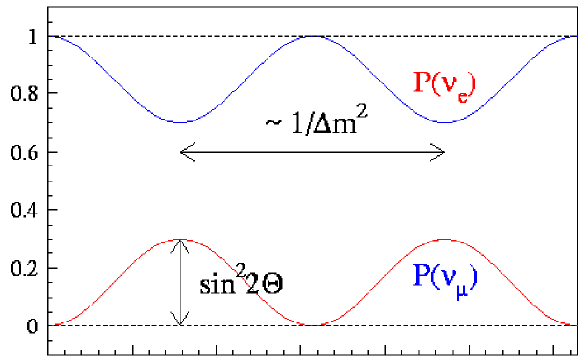
\includegraphics[width=0.6\linewidth]{neutrinos/neutrino_osc.png}
    \caption{Plot van de neutrino flavour waarschijnlijkheden}%
    \label{fig:neutrinos/neutrino_osc}
\end{figure}

\subsection{Oscillaties: 3 generaties}%
\label{sub:oscillaties_3_generaties}

Voegen we nu de 3de generatie aan neutrinos toe. Dit zal ons in de plaats van de eenvoudige $2\times 2$ opmenging matrix nu een $3\times 3$ matrix geven tussen de flavour eigentoestanden en de massa eigentoestanden.
\begin{equation}
    \begin{aligned}
        \label{eq:neutrino_3_oscilaties_1}
\left|\nu_{\alpha}\right> &=\sum_{i} U_{\alpha i}\left|\nu_{i}\right> \\
        U &=\left(\begin{array}{lll}
                U_{\alpha 1} & U_{\alpha 2} & U_{\alpha 3} \\
                U_{\beta 1} & U_{\beta 2} & U_{\beta 3} \\
                U_{\gamma 1} & U_{\gamma 2} & U_{\gamma 3}
        \end{array}\right)
    \end{aligned}
\end{equation}
Deze matrix kan op een gelijkaardige manier geparametriseerd worden als de CKM-matrix. De naam van deze matrix is de ``Pontecorvo-Maki-Nakagawa-Sakata (PMNS) matrix''.
\begin{equation}
    \begin{aligned}
        \label{eq:pmns_matrix}
        U=\left(\begin{array}{ccc}
                c_{12} c_{13} & s{12} c_{13} & s_{13} e^{-i \delta} \\
                -s_{12} c_{23}-c_{12} s_{23} s_{13} e^{i \delta} & c_{12} c_{23}-s_{12} s_{23} s_{13} e^{i \delta} & s_{23} c_{13} \\
                s_{12} s_{23}-c_{12} c_{23} s_{13} e^{i \delta} & -c_{12} s_{23}-s_{12} c_{23} s_{13} e^{i \delta} & c_{23} c_{13}
        \end{array}\right)
    \end{aligned}
\end{equation}
Hierbij zijn $c_{i j}=\cos \theta_{i j}$, $s_{i j}=\sin \theta_{i j}$ en $\delta$ de $CP$-schende fase. Ook zoals bij de CKM-matrix is het mogelijk om de PMNS-matrix te herschrijven als volgt:
\begin{equation}
    \begin{aligned}
        \label{eq:pmns_matrix_ontbonden}
        U =&\left(\begin{array}{ccc}
                1 & 0 & 0 \\
                0 & c_{23} & s_{23} \\
                0 & -s_{23} & c_{23}
                \end{array}\right) \times\left(\begin{array}{ccc}
                c_{13} & 0 & s_{13} e^{-i \delta} \\
                0 & 1 & 0 \\
                -s_{13} e^{i \delta} & 0 & c_{13}
        \end{array}\right) \\
        &\times\left(\begin{array}{ccc}
                c_{12} & s_{12} & 0 \\
                -s_{12} & c_{12} & 0 \\
                0 & 0 & 1
                \end{array}\right) \times\left(\begin{array}{ccc}
                e^{i \alpha_{1} / 2} & 0 & 0 \\
                0 & e^{i \alpha_{2} / 2} & 0 \\
                0 & 0 & 1
        \end{array}\right)
    \end{aligned}
\end{equation}
We zien dat er voor de neutrinos extra $CP$ schendende termen ($\alpha_1$ en $\alpha_2$) moeten toegevoegd worden aan de matrix indien het Majorana deeltjes zouden zijn. Al dit zal ons iets meer ingewikkelde waarschijnlijkheden geven waar de sinussen en cosinussen vervangen zijn door de PMNS-matrix elementen.
\begin{equation}
    \begin{aligned}
        \label{eq:neutrino_3_oscilaties_2}
        P_{\nu_{\alpha} \rightarrow \nu_{\beta}} &=\left|\left<\nu_{\beta}(t)\mid \nu_{\alpha}(t=0)\right>\right|^{2} \\
                                                 &=\delta_{\alpha \beta}-4 \sum_{j>i} U_{\alpha i} U_{\beta i} U_{\alpha j} U_{\beta j} \sin ^{2}\left(\frac{\Delta m_{i j}^{2} L}{4 E_{\nu}^{\nu}}\right)
    \end{aligned}
\end{equation}
met $U_{\alpha i}$ reëel als $\delta=0$ is. Wat we opmerken is dat we een sinus kwadraat hebben en dus ongevoelig zijn voor het teken van $\Delta m^2$. Het zal dus mogelijk zijn om het verschil in massa tussen 2 neutrino flavours te bepalen maar het is niet mogelijk om te zeggen welke de lichtste zal zijn.

\subsection{MSW effect}%
\label{sub:msw_effect}

We willen eigenlijk echt wel weten welk neutrino welke massa heeft. Om dit probleem op te lossen is het hebben van een materie effect. Als we de neutrinos nu eens laten propageren door materie in plaats van een vacuum zal deze interageren met die materie, in het bijzonder de elektronen. Naast de gewone elastische botsingen krijgen we naast de neutrale stroom ook een geladen stroom interactie.

\begin{figure}[h]
    \centering
    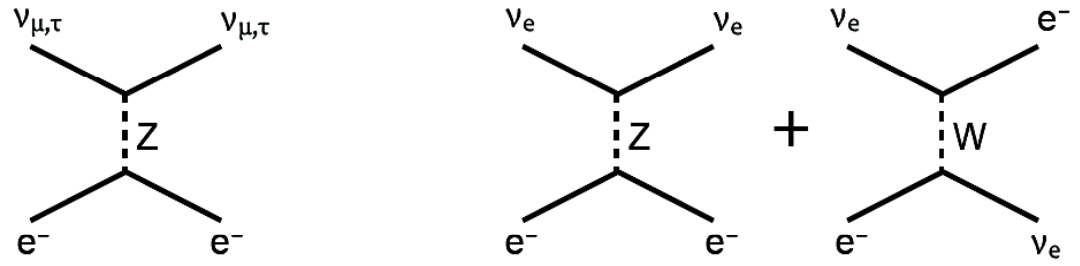
\includegraphics[width=0.7\linewidth]{neutrinos/msw_effect_diagrammen.png}
    \caption{Feynman diagrammen van mogelijke neutrino reacties in materie}%
    \label{fig:neutrinos/msw_effect_diagrammen}
\end{figure}

Zoals dat de $W$ en $Z$ bosonen massa krijgen door te interageren met het Higgs veld en zo inertie te krijgen en de protonen die een wolk van quarks en gluonen om zich heeft, zullen de neutrinos constant met het zwakke interactieveld interageren en creëren zo een wolk van elektronen, $Z$ bosonen en $W$ bosonen rond zich hebben. Deze wolk interageerd met de elektronen in de materie en krijgen een effectieve massa. Dit zal zich vertonen als een aanpassing van de massaterm in de oscillaties.
\begin{equation}
    \begin{aligned}
        \label{eq:msw_effect}
        \Delta m_{M}^{2}&=\Delta m^{2} \times \xi\\
        \xi&=\sqrt{\sin ^{2}(2 \theta)+\left(\cos (2 \theta)-\frac{A_{C C}}{\Delta m^{2}}\right)^{2}}\\
        \sin \left(2 \theta_{M}\right)&=\frac{\sin (2 \theta)}{\xi}\\
        A_{C C}&=\pm 2 \sqrt{2} E_{\nu} G_{F} N_{e}
    \end{aligned}
\end{equation}
In deze aanpassing zit de afhankelijkheid van de charged current reactie, $A_{CC}$. In deze term zit natuurlijk de zwakke wisselwerking constante en een gevoeligheid voor de densiteit aan elektronen in. De reden voor $\pm$ in $A_{CC}$ is dat de charged current interactie ook kan gebeuren in een t-channel met antineutrinos.\\
\begin{center}
    \feynmandiagram[horizontal=a to b]{
        i2 [particle=\(e^{-}\)] -- [fermion] a -- [fermion] i1 [particle=\(\bar{\nu}_e\)],
        a -- [boson, edge label=\(W^-\)] b,
        f1 [particle=\(\bar{\nu}_e\)] -- [fermion] b -- [fermion] f2 [particle=\(e^-\)],
    };
\end{center}
Hier kan mee aan de slag gegaan worden. We hebben een maximale mixing ($\sin \left(2 \theta_{M}\right)=1$) als $A_{C C}=\Delta m^{2} \cos (2 \theta)$ is. Zo krijgen we de afhankelijkheid van de elektron densiteit
\begin{equation}
    \begin{aligned}
        \label{eq:msw_elektron_densiteit}
        N_{e}^{R}=\frac{\Delta m^{2} \cos (2 \theta)}{2 \sqrt{2} E_{\nu} G_{F}}
    \end{aligned}
\end{equation}
die bij de energie van het neutrino een resonantiepiek zal hebben. Het mooie is dat we hierbij gevoelig zijn voor het teken van massa kwadraat verschil. Dit kunnen we nu dus meten.

\begin{figure}[h]
    \centering
    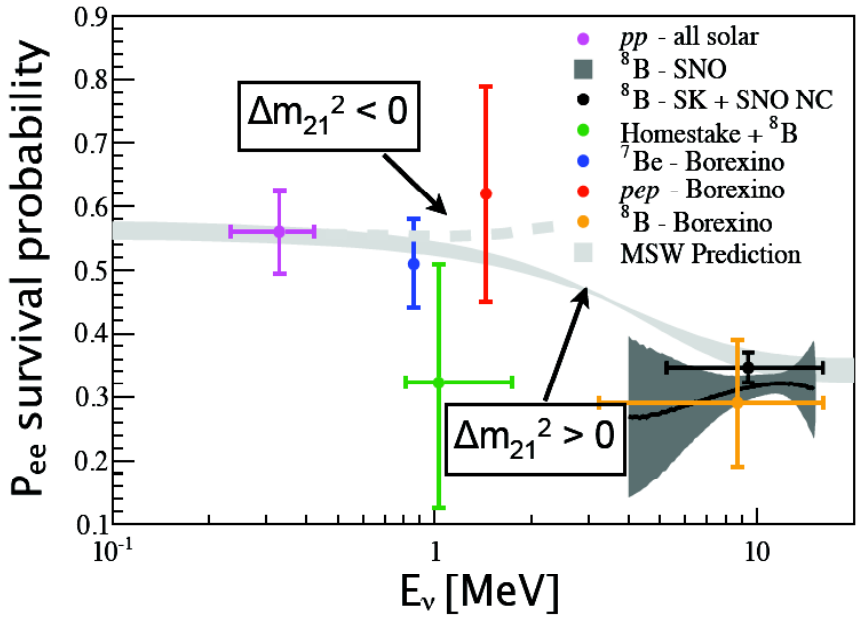
\includegraphics[width=0.5\linewidth]{neutrinos/msw_resultaten.png}
    \caption{Resultaten voor het massaeffect}%
    \label{fig:neutrinos/msw_resultaten}
\end{figure}

Hierbij bekijken we de survival probabiliteit van de elektron neutrinos in functie van hun energie. Het verschil in de hoeveelheid waargenomen neutrinos bij de verschillende experimenten kan nu begrepen worden. De hoeveelheid neutrinos dat wordt waargenomen hangt af van de energie waarbij we deze waarnemen. Hier kunnen we nu dus uit bepalen welk neutrino zwaarder is. Omdat de waarschijnlijkheid afneemt bij hogere energie wil dit zeggen dat de 2de massa eigentoestand zwaarder zal zijn dan de eerste.

\subsection{Bepalen van $\theta_{12}, \Delta m_{21}^{2}$}%
\label{sub:bepalen_van_de_parameters}

\begin{figure}[h]
    \centering
    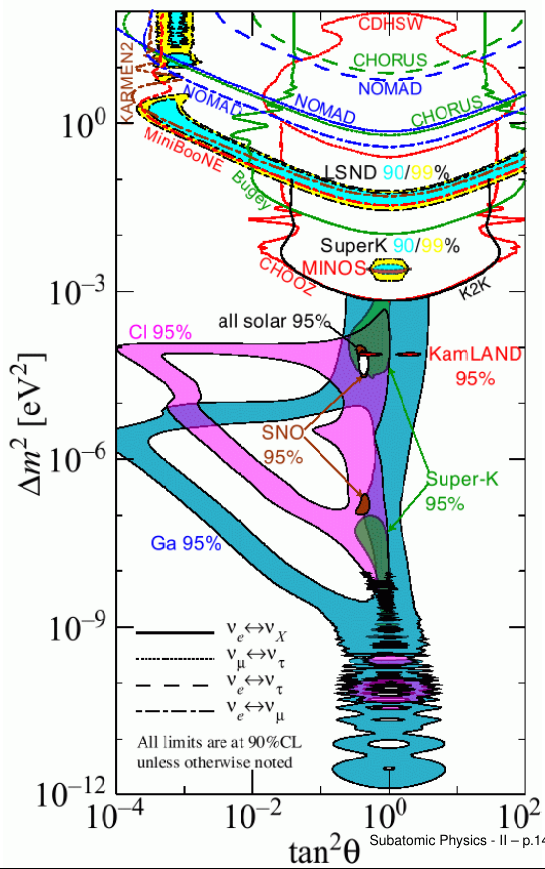
\includegraphics[width=0.6\linewidth]{neutrinos/alle_neutrino_resultaten.png}
    \caption{Samenvoeging van een groot deel van van de neutrino experimenten}%
    \label{fig:neutrinos/alle_neutrino_resultaten}
\end{figure}

Na al dit meten is het nu mogelijk om $\theta_{12}$ en $\Delta m_{21}^{2}$ te bepalen. Dit doen we aan de hand van de experimenenten op zonne neutrinos en het Kamiokande experiment. Als deze overeen zouden komen is de $CP$ behouden. Bekijken we al deze experimenten samen zien we dat elke in het centrale gebied de metingen overeen zullen komen met elkaar. Vandaag de dag hebben we voor deze parameters de volgende waarden:
\begin{equation}
    \begin{aligned}
        \label{eq:neutrino_osc_waarden}
        \Delta m_{21}^{2}&=m_{2}^{2}-m_{1}^{2}=(7.6 \pm 0.2) \times 10^{-5} \mathrm{eV}^{2}\\
        \sin ^{2}\left(2 \theta_{12}\right)&=0.87 \pm 0.04
    \end{aligned}
\end{equation}
Wat dit ons zegt is dat 1 van de 2 massa moeten hebben. Het is dus perfect mogelijk dat één van de 2 een massa van 0 heeft.

\subsection{2de generatie}%
\label{sub:2de_generatie}

De $\mu$ en $\tau$ neutrinos kunnen ook opmengen met elkaar. Dit hoeft eigenlijk niet dus onderzoeken we dit. Om dit te onderzoeken kijken we naar atmosferische neutrinos. Deze bestaan vooral uit $\nu_\mu$ omdat de gecreëerde pionen in de atmosfeer vervallen tot muonen en zijn neutrinos. Zoals gewoonlijk is het moeilijk om deze te detecteren. Zelf neutrinos van de andere kant van de aarde zijn in staat om aan het experiment te komen. Deze hoog energetische neutrinos zijn voor het eerst waargenomen in 2005 in het SuperKamiokande experiment. Figuur \ref{fig:neutrinos/superkamiokande_experiment} geeft de resultaten van dit experiment terug.

\begin{figure}[h]
    \centering
    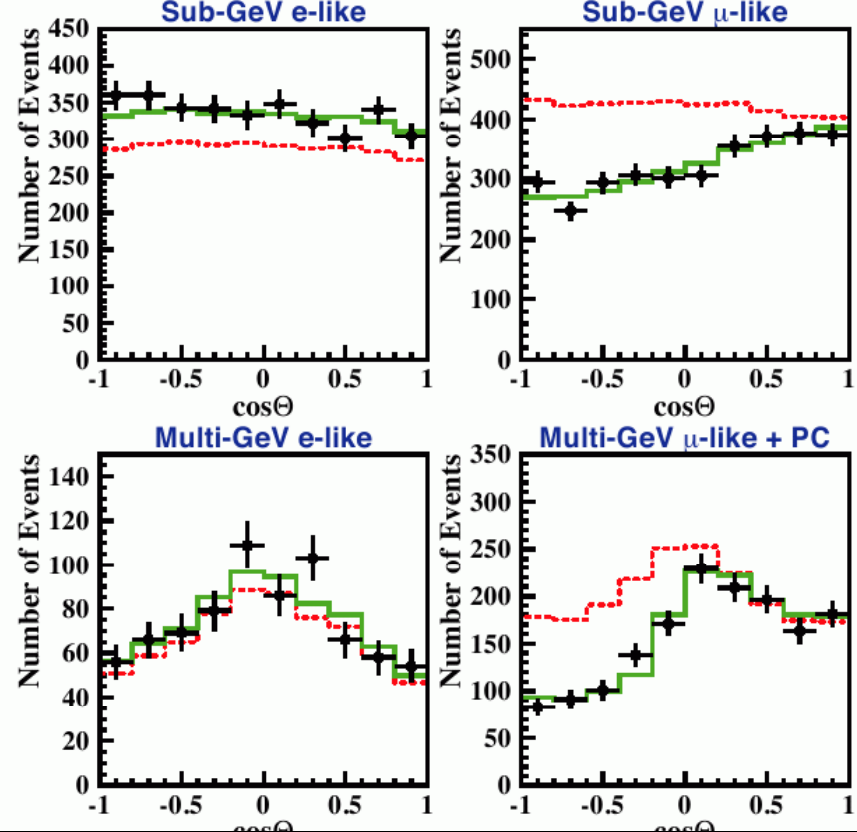
\includegraphics[width=0.5\linewidth]{neutrinos/superkamiokande_experiment.png}
    \caption{Resultaten van SuperKamiokande voor atmosferische neutrinos}%
    \label{fig:neutrinos/superkamiokande_experiment}
\end{figure}

Het is mogelijk om een onderscheidt te maken tussen elektron en muon neutrinos aan hoe diffuus de Cherenkov ring is. De elektronen ring is door de vele interacties veel deffuser dan de muon ring die tientallen meters kan afleggen voor deze interageert. In de resultaten worden het aantal events uitgezet in functie van de invalshoek met $\Theta = 1$ deeltjes die van bovenaf komen en $\Theta = -1$ deeltjes die van beneden komen en dus eerst door de aarde zijn gegaan. Voor de elektron neutrinos zien we dat de voorspellingen vrij goed worden gevolgd maar bij de laag energetische elektron neutrinos zien we over het algemeen een 10tal percent meer elektronen dan verwacht (komt van muon oscillatie naar $\tau$ neutrinos en dan naar elektron neutrinos). Voor de muon neutrinos zien we iets totaal anders. In zowel hoog als laag energetische muon neutrinos zien we voor deze die door de aarde gaan maar de helft die we verwachten. Deze zijn duidelijk geoscilleerd in neutrinos met een andere flavour. Deze afwijkingen wijzen er op de de muon neutrinos vooral in $\tau$ neutrinos zullen oscilleren omdat we geen overmaat zien in de elektron neutrinos. De reden waarom dat elektron neutrinos niet oscilleren is omdat ze nog niet genoeg tijd hebben gehad om te oscilleren, de muon neutrinos blijkbaar wel. Kijken we terug naar de relatie gegeven in vergelijking (\ref{eq:neutrino_2_oscilaties_7}) is dit verschil hier omdat het massaverschil bij de muon neutrinos groter zal zijn dan bij de elektron neutrinos. De hoek tussen de eerste en 3de generatie $\theta_{13}$ zal dus klein moeten zijn omdat de percentuele afwijking van de elektron neutrino waarnemingen klein is.\\
In de resultaten van IceCube zien we sterke oscillaties met $\sin^2(2\theta_{23})$ van de orde 1 en massaverschillen tussen de 2de en derde generatie van $2\times 10^{-3}\text{eV}^2$. We merken direct op dat de nauwkeurigheid hier een pak minder is vanwege de moeilijkheidsgraad om deze te detecteren.

\begin{figure}[h]
    \centering
    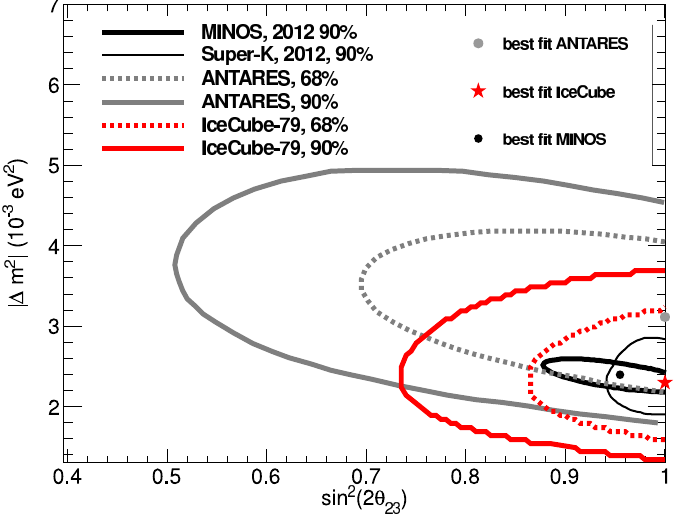
\includegraphics[width=0.5\linewidth]{neutrinos/icecube.png}
    \caption{Resultaten van het IceCube experiment}%
    \label{fig:neutrinos/icecube}
\end{figure}

Vandaag de dag hebben we de volgende resultaten:
\begin{equation}
    \begin{aligned}
        \label{eq:neutrino_osc_waarden_vervolg}
        \left|\Delta m_{32}^{2}\right|&=\left|m_{3}^{2}-m_{2}^{2}\right|=(2.3 \pm 0.1) \times 10^{-3} \mathrm{eV}^{2} \\
        \Delta m_{21}^{2}=m_{2}^{2}-m_{1}^{2}&=(7.6 \pm 0.2) \times 10^{-5} \mathrm{eV}^{2} \\
        \sin ^{2}\left(2 \theta_{23}\right)&>0.92 \\
        \sin ^{2}\left(2 \theta_{12}\right)&=0.87 \pm 0.04
    \end{aligned}
\end{equation}
De massa van de derde generatie aan neutrinos zal duidelijk groter zijn dan deze van de eerste en 2de generatie en de amplitude tussen de tweede en derde generatie is met ongeveer 1 te zijn vrij hoog. Dit zien we niet bij de quarks waar we naar heel kleine effecten moeten kijken om de oscillaties waar te nemen.

\subsection{Relatie tussen eerste en derde generatie}%
\label{sub:relatie_tussen_eerste_en_derde_generatie}

Uit vorig experiment hebben we gezien dat de amplitude $\theta_{13}$ tussen de eerste en derde generatie heel klein moet zijn. Met andere woorden zou er geen $CP$ schending mogen zijn. Je hebt opmengen van deze 2 generaties nodig om $CP$ schending te laten optreden. Hoe kunnen we die $CP$ schending nu gaan meten? Dit doen we aan de hand van figuur \ref{fig:neutrinos/neutr_osc_waarschijnlijkheid}. Hier bekijken we de waarschijnlijkheid dat een elektron neutrino zal oscilleren naar een andere flavour in functie van de afstand/energie.

\begin{figure}[h]
    \centering
    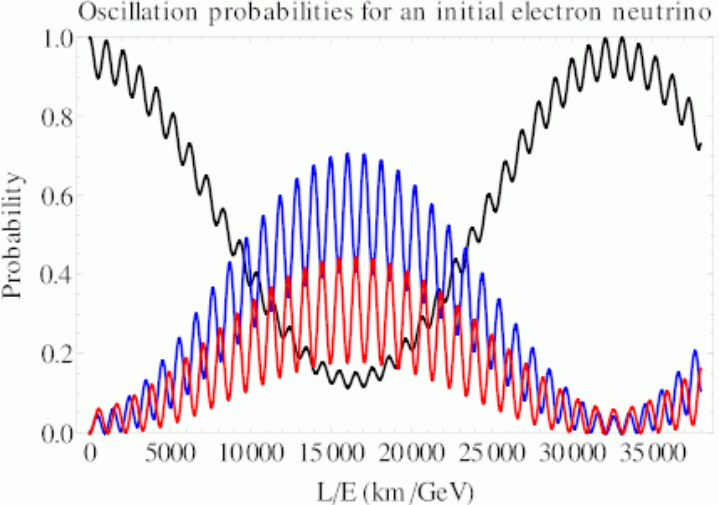
\includegraphics[width=0.6\linewidth]{neutrinos/neutr_osc_waarschijnlijkheid.png}
    \caption{Waarschijnlijkheid dat een elektron neutrino oscilleert in een andere flavour}%
    \label{fig:neutrinos/neutr_osc_waarschijnlijkheid}
\end{figure}

Hier kunnen we oscillatie frequenties uit halen. De ene is een oscillatie met grote amplitude en lage frequentie van de orde $15000L/E$ in $\mu$ en $\tau$ neutrinos, dit is de oscillatie tussen de eerste en 2de generatie. Dan hebben we ook een oscillatie tussen de eerste en 3de generatie die een veel hogere frequentie die vergelijkbaar is met de frequentie tussen de 2de en 3de generatie. Omdat de energie van de neutrinos te laag is, is het voor de muon en $\tau$ neutrinos niet mogelijk om muonen of $\tau$'s aan te maken en is het niet mogelijk om de blauwe en rode functies te onderscheiden.\\
Om $\theta_{13}$ waar te kunnen nemen moeten we in de plaats van te kijken over afstanden van honderden kilometers gaan kijken over een afstand van een aantal kilometer. In 2010 wordt hier onderzoek naar gedaan waar 3 verschillende detectoren op verschillende afstanden van 4 verschillende reactoren worden geplaatst. Uit deze experimenten was duidelijk dat $\nu_e$ oscilleert in $\nu_\tau$ over deze kleine afstand. 

\begin{figure}[h]
    \centering
    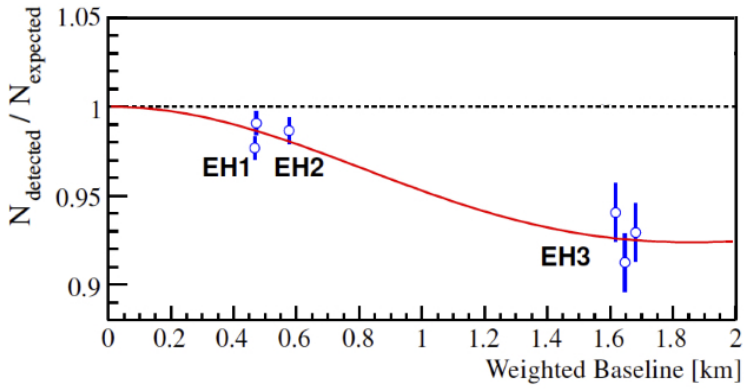
\includegraphics[width=0.6\linewidth]{neutrinos/1_3_oscillatie.png}
    \caption{Onderzoek naar $CP$ schending bij neutrinos}%
    \label{fig:neutrinos/1_3_oscillatie}
\end{figure}

Na 1.5km kan je zien dat er een kleine oscillatie van elektron naar $\tau$ neutrinos zal plaats gevonden hebben. Vandaag de dag weten we dat het massaverschil tussen de eerste en derde generatie en tussen tweede en derde generatie gelijk zijn omdat het massaverschil tussen de eerste en tweede generatie verwaarloosbaar klein is. De mengingshoek in tegenstelling tot de andere mengingshoeden zal hier klein zijn $\sin ^{2}\left(2 \theta_{13}\right) \approx 0.10 \pm 0.01$.

\subsection{PMNS matrix}%
\label{sub:pmns_matrix}

De PMNS-matrix ziet er nu als het volgt uit:
\begin{equation}
    \begin{aligned}
        \label{eq:pmns_matrix_ingevuld}
        \left(\begin{array}{ccc}
                \left|U_{e 1}\right| & \left|U_{e 2}\right| & \left|U_{e 3}\right| \\
                \left|U_{\mu 1}\right| & \left|U_{\mu 2}\right| & \left|U_{\mu 3}\right| \\
                \left|U_{\tau 1}\right| & \left|U_{\tau 2}\right| & \left|U_{\tau 3}\right|
                \end{array}\right) \approx\left(\begin{array}{ccc}
                0.85 & 0.50 & 0.17 \\
                0.35 & 0.60 & 0.70 \\
                0.35 & 0.60 & 0.70
        \end{array}\right)
    \end{aligned}
\end{equation}
We zien hier dat de eerste en 2de generatie vrij sterk opmengen met waarden $0.5$ en $0.35$, dat de 2de en 3de generatie ook sterk opmengen met waarden $0.7$ en $0.6$ en ten laatste zien we dat de eerste en 3de generatie het minst zullen opmengen maar veel meer dan de opmenging in de quark sector met waarden $0.35$ en $0.17$. We zien dat deze matrix bijna vlak is met grote opmengingshoeken $\theta_{12} \approx 35^{\circ}$, $\theta_{23} \approx 45^{\circ}$ en $\theta_{13} \approx 10^{\circ}$. Het is hier dus mogelijk dat er $CP$ schending zou zijn omdat $\theta_{13} \neq 0$. De vraag is nu of deze PMNS-matrix unitair is. Binnen de grote foutenmarges die we op dit moment hebben is deze matrix perfect unitair. De volgende vraag is natuurlijk wat de $CP$ schendende fase is. Hiervoor moeten we natuurlijk kijken naar de $CP$ schending van de neutrino oscillaties wat een probleem is.

\subsection{Neutrino massa hiërarchie}%
\label{sub:neutrino_massa_hierarchie}

Het eerste probleem waar we naar kijken is de $\Delta m_{32}^2$ waar we het teken nog niet van hebben kunnen vast leggen. Voor de eerste en 2de generatie hebben we het teken gemeten aan de hand van het massaeffect wat niet mogelijk is bij deze generaties. Er zijn dus 2 mogelijkheden voor de massa hiërarchieën weergegeven in figuur \ref{fig:neutrinos/massa_hier}. Dit zijn de normale en inverse hiërarchie.

\begin{figure}[h]
    \centering
    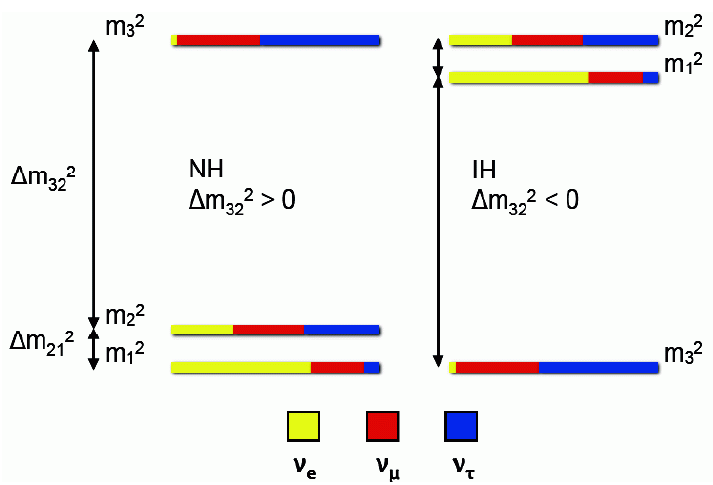
\includegraphics[width=0.5\linewidth]{neutrinos/massa_hier.png}
    \caption{Mogelijke massa hiërarchieën voor de verschillende neutrinos}%
    \label{fig:neutrinos/massa_hier}
\end{figure}

Hier kan je ook zien dat je niet zal kunnen zeggen welke flavour toestanden nu het zwaarst zijn. We kunnen alleen iets zeggen over de massa eigentoestanden.

\subsection{Neutrino oscillaties in IceCube}%
\label{sub:neutrino_oscillaties_in_icecube}

Om het massaverschil tussen de 2de en 3de generatie te bepalen maken we weer gebruik van een massaeffect, deze keer tussen de $\mu$ en $\tau$ neutrinos. Eén van de experimenten die daar zeer gevoelig voor zijn is het IceCube experiment. Dit is een grote neutrino detector in het ijs aan de zuid pool. Naast de neutrinos te bekijken die boven de zuidpool zijn gemaakt, is het ook mogelijk om neutrinos door de aarde waar te nemen. Zo is het mogelijk afhankelijk van waar op de aarde de muon neutrinos binnen komen een andere hoeveelheid materiaal zullen doorkruist hebben voor ze gedetecteerd worden.

\begin{figure}[h]
    \centering
    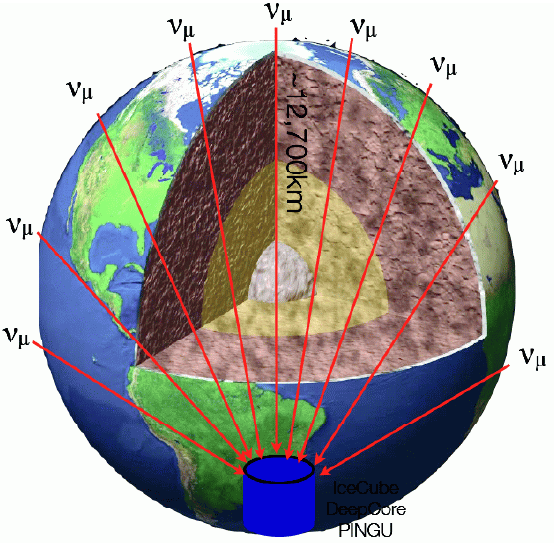
\includegraphics[width=0.3\linewidth]{neutrinos/icecube_voorstelling.png}
    \caption{Voorstelling van verschillende muon paden door de aarde naar IceCube}%
    \label{fig:neutrinos/icecube_voorstelling}
\end{figure}

In dit experiment worden neutrinos over grote energie ranges en padlengtes bekeken wat escentieel is voor de systematische controle. Het is nu mogelijk om dit in detail te gaan bekijken. Voor afstanden van de diameter van de aarde zal het eerste minimum in $P\left(\nu_{\mu} \rightarrow \nu_{\mu}\right)$ (de verdwijning van de muon neutrinos) rond de energie van $E_\nu \approx 25$GeV liggen.

\begin{figure}[h]
    \centering
    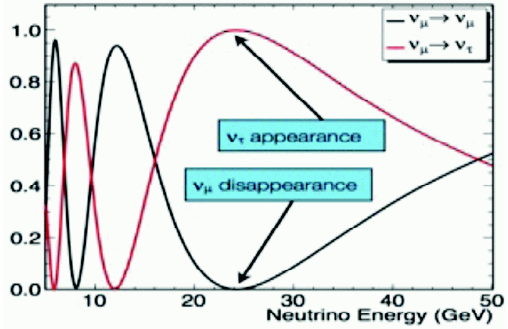
\includegraphics[width=0.5\linewidth]{neutrinos/muon_tau_neutr_osc.png}
    \caption{Neutrino waarschijnlijkheden in functie van hun energie}%
    \label{fig:neutrino}
\end{figure}

Op hetzelfde moment zouden dan ook $\tau$ neutrinos waargenomen moeten kunnen worden wat heel moeilijk is.\\
Waar komt het massaeffect nu aan te pas? Voor neutrinos die schuin binnen komen en enkel door de mantel van de aarde gaan zal het massa effect vrij klein moeten zijn en is het verschil tussen de normale en geïnverteerde hiërarchie vrij klein. Anderzijds is het ook mogelijk dat de neutrinos dwars door de aarde gaan en dus ook door de heel dense kern van de aarde gaat en dus een heel ander effect zullen zien. We zullen tussen de 2 hiërarchieën dus 2 heel andere oscillaties waarnemen. Om dit te doen moet heel het model doorgerekend worden. We verwachten om binnen 5 jaar hier meer over te weten.

\subsection{$CP$ schending}%
\label{sub:_cp_schending_neutrinos}

Het meten van de $CP$ schending doen we aan de hand van het verschil wat neutrinos doen en wat antineutrinos doen. Je kijkt dus naar de oscillatie van elektron neutrinos in muon neutrinos en van elektron antineutrinos in muon antineutrinos.
\begin{equation}
    \begin{aligned}
        \label{eq:cp_schending_neutrinos_1}
        P\left(\nu_{e} \rightarrow \nu_{\mu}\right)-P\left(\bar{\nu}_{e} \rightarrow \bar{\nu}_{\mu}\right)
    \end{aligned}
\end{equation}
Uit de zon is het mogelijk om de elektron neutrinos te onderzoeken en de anti elektron neutrinos kunnen onderzocht worden bij reactoren. Met de fouten die we hebben op onze experimenten, kunnen we zien dat de experimenten ten hoogste een paar percent is (dit is enkel een boven limiet). Dit is heel veel in vergelijking tot de quark sector waar het gaat over enkele promille.\\
Een beter experiment is het onderzoeken van een $\nu_\mu$-beam experiment waar het gemakkelijk is om $\nu_\mu$ en $\bar{\nu}_\mu$ aan te maken. Deze bundels kunnen gemaakt worden uit het verval van $\pi^\pm \rightarrow \mu^\pm + \bar{\nu}_\mu/\nu_\mu$. Met de mogelijkheid om te bepalen wat de dominant is (neutrinos of antineutrinos) is het mogelijk om de oscillatie van muon (anti)neutrinos in elektron (anti)neutrinos te bekijken.
\begin{equation}
    \begin{aligned}
        \label{eq:cp_schending_neutrinos_2}
        P\left(\nu_{\mu} \rightarrow \nu_{e}\right)-P\left(\bar{\nu}_{\mu} \rightarrow \bar{\nu}_{e}\right)
    \end{aligned}
\end{equation}
De resultaten van een paar jaar geleden zijn in figuur \ref{fig:neutrinos/t2k} te vinden. Daar wordt $\delta_{CP}$ in functie van $\sin ^{2} 2 \theta_{13}$ gegeven.

\begin{figure}[h]
    \centering
    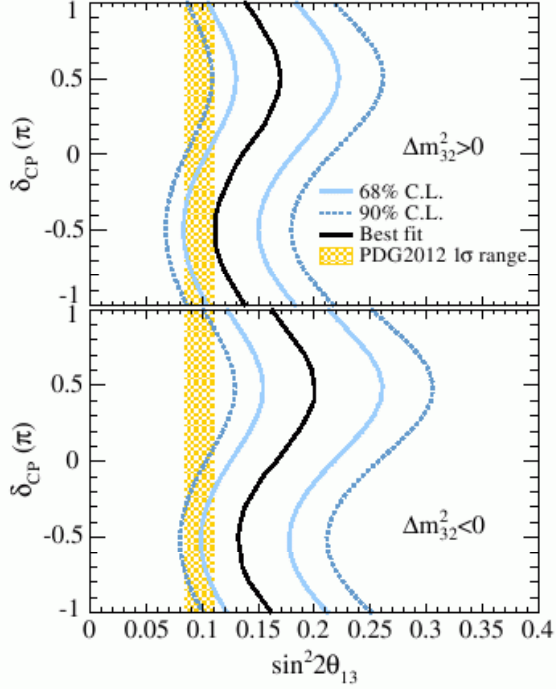
\includegraphics[width=0.4\linewidth]{neutrinos/t2k.png}
    \caption{Resultaten uit het T2K}%
    \label{fig:neutrinos/t2k}
\end{figure}

Voor $\Delta m_{32}^{2}<0$ krijgen we $CP$ schending van de orde $-0.5$ wat 90 graden is. Voor $\Delta m_{32}^{2}>0$ ziet dit er ook zo uit. Deze ondervindingen zijn een aantal weken geleden geüpdatet en worden de eerdere waarden bevestigd (figuur \ref{fig:neutrinos/t2k_update}).

\begin{figure}[h]
    \centering
    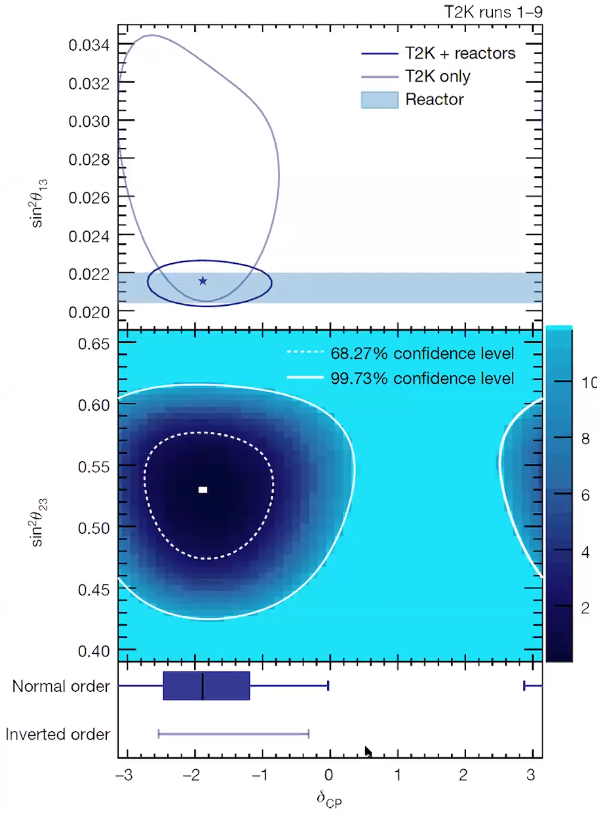
\includegraphics[width=0.4\linewidth]{neutrinos/t2k_update.png}
    \caption{Geüpdatet waarden uit het T2K}%
    \label{fig:neutrinos/t2k_update}
\end{figure}

Zoals je kan zien aan de fouten vlaggen zijn dit enkel nog maar aanwijzingen. ``Alles'' is nog mogelijk. Op dit moment lijkt het er gewoon op dat er veel $CP$ schending zit in de neutrino sector en is binnen de komende jaren meetbaar.\\
De reden waarom de $CP$ schending in de lepton sector zo belangrijk is, is omdat we op dit moment denken dat bij de big bang het universum eerst een leptogenese is ondergaan voor een baryogenese. We denken dat het onderscheidt tussen materie en antimaterie eerst is gemaakt in de lepton sector, niet de quark sector. Deze leptonen zijn dan aan de hand van $CP$ schending en het \href{https://en.wikipedia.org/wiki/Sphaleron}{sphaleron effect} deels omgezet in baryonen.

\subsection{Dirac vs Majorana}%
\label{sub:dirac_vs_majorana}

Het vreemde aan de neutrinos is dat we enkel rechts handige neutrinos hebben, geen links handige. Alle andere fermionen in het Standaard Model zijn Dirac deeltjes. Dit betekent dat deze zowel links als rechts handig zijn, $f_{R}, f_{L}, \bar{f}_{R}, \bar{f}_{L}$. Indien de massa van het fermion groter is dan 0 zou het altijd mogelijk moeten zijn om een rechtshandig fermion aan de hand van een Lorentz boost om te zetten in een linkshandig fermion. Dit kan niet gedaan worden voor deeltje antideeltjes. Voor de neutrinos met een massa zo goed als nul hebben we maar 2 staten geobserveerd: $\nu_L$ en $\bar{\nu}_R$. Dit zijn natuurlijk verschillende objecten.\\
In 1937 stelt Majorana een andere theorie voor die ook zal werken om neutrale deeltjes te beschrijven die heel goed zal lijken op de Dirac vergelijking. In de vergelijking van Majorana zullen de deeltjes en antideeltjes gelijk zijn aan elkaar.
\begin{equation}
    \begin{aligned}
        \label{eq:majorana_deeltjes}
        f &= \bar{f}\\
        \nu_L &= \bar{\nu}_L\\
        \nu_R &= \bar{\nu}_R\\
    \end{aligned}
\end{equation}
Voor deeltjes met massa gelijk aan 0 zal er geen verschil zijn tussen de Dirac en Majorana deeltjes. Indien de deeltjes wel massa hebben zal het wel mogelijk zijn om een onderscheidt te gaan maken en is het mogelijk om te werken met de eerder aangehaalde Lorentz boost. In de linkshandige neutrino zal een stuk rechtshandige component zitten m.a.w. zal daar een stuk antineutrino inzitten.\\
Kijken we nu eens naar het verval van een pion in onderandere een neutrino.
\begin{equation}
    \begin{aligned}
        \label{eq:pion_neutrino_verval}
        \pi^{+} \rightarrow \mu^{+} \nu_{\mu}
    \end{aligned}
\end{equation}
In het Standaard Model is het hat enkel mogelijk om het neutrino waar de nemen aan de hand van de volgende interactie: $\nu_{\mu} n \rightarrow \mu^{-} p$. Indien neutrinos Majorana deeltjes zijn, zou het mogelijk zijn dat de rechtshandige component zich voordoet als $\bar{\nu}_\mu$ die dan ook kan interageren met een proton: $\nu_M P \longrightarrow \mu^{+} n$. Dit is echter maar een heel kleine component. Deze reactie van die mogelijk zou zijn met Majorana neutrinos, zal het lepton getal niet behouden $\Delta \mathcal{L}=-2$. Door maar een heel kleine component aan linkshandige antideeltjes te hebben zal dit een heel klein effect zijn, $O\left(m_{\nu}^{2} / m_{\mu}^{2}\right) \sim 10^{-22}$.

\end{document}
